\documentclass[../main.tex]{subfiles}
\begin{document}
\subparagraph{Simulation 6.d}\label{subpar:sim_6_d}

$c_{9}=0.8$ and $|g(t_{\text{end}})| = 0.6409$.

\begin{figure}[H]
    \centering 
    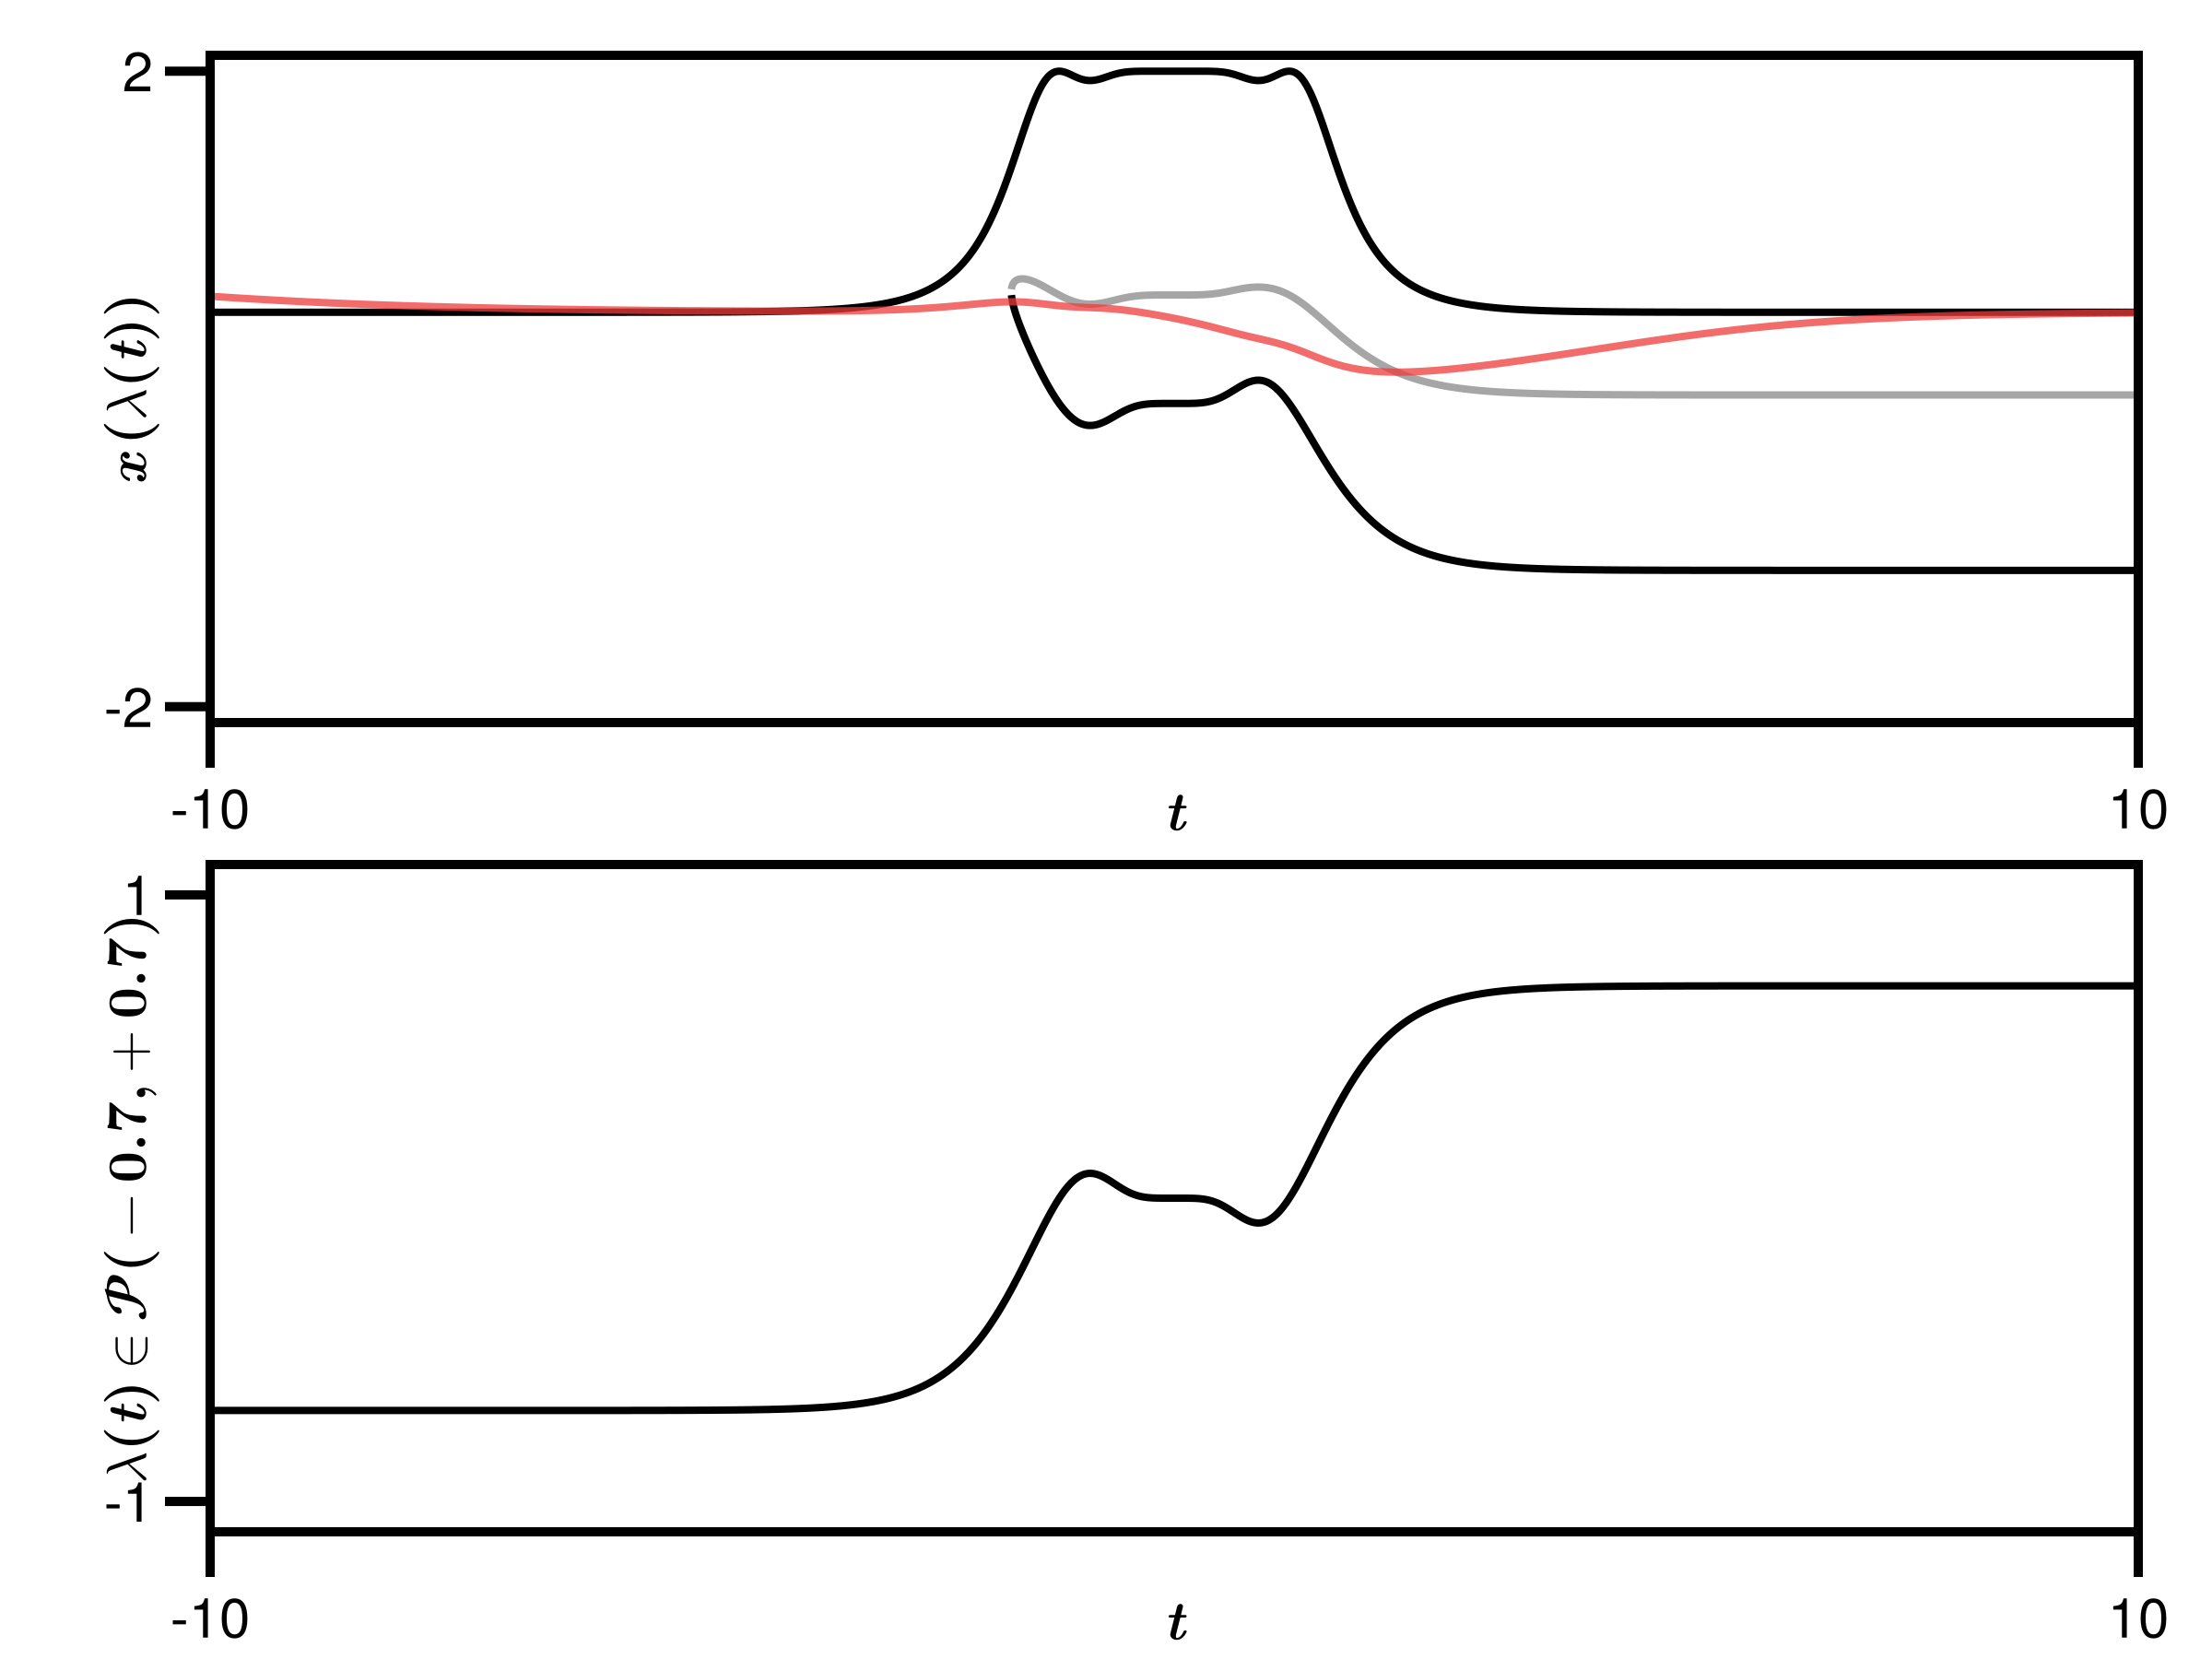
\includegraphics[keepaspectratio, width=\textwidth]{../figures/sim_6.d.png}
    \caption{Solution of \eqref{eq:dyn_sys} (top) with the parameter shift \eqref{eq:sim_6_shift} (bottom). No R-tipping.}
    \label{fig:sim_6_d}
\end{figure}

\end{document}
